\section{Introduction}

\subsection{Problem Statement}
Modern deep learning algorithms have been shown to improve performance for tasks such as classification, segmentation and detection in digital pathology. However, deep learning algorithms require large annotated datasets from which to build high performing models. This requirement for data has been identified as a key challenge for using deep learning algorithms for digital pathology~\cite{tizhoosh2018artificial} and medical image analysis~\cite{geert2017survey}. There are several approaches to tackling this problem which include semi-supervised learning, weakly supervised learning, active learning, and their combinations. This paper focuses on the use of active learning to aid in annotation collection for patch-based digital pathology image analysis.

Active learning is a type of machine learning which hypothesises that having a learning algorithm select the data it uses to train itself can reduce the amount of data needed for training. Active learning is used within modern applications to reduce the quantity of annotations needed. Annotating only the data selected by the learning algorithm reduces the overall cost of building an effective model. In a pool-based scenario, the learning algorithm has access to a large pool of unannotated data. Over multiple iterations, the learning algorithm selects data to be annotated and added to the training data ~\cite{settles2012active}.

Active learning algorithms use query strategies to select the data to be annotated. There are numerous query strategies available with the most popular methods being based on uncertainty. Uncertainty sampling is a simple query strategy that samples data based on a model’s predictions for the unannotated data.

While these methods have been shown to work well with many  traditional learning algorithms, this is not the case when working with deep learning algorithms. There are several reasons for this. Firstly, deep learning algorithms jointly learn feature representations and classifiers/regressors. Selecting only difficult examples to train the model leads to learnt features that are not representative, decreasing the quality of the model ~\cite{wang2018ceal}. Secondly, traditional query strategies are used to select a single data point. It has been shown that deep learning algorithms work better with batch updates and so require a query strategy to select an optimal batch and not just the top ranked points ~\cite{sener2018active}. Thirdly, the softmax output from a classifier trained using deep learning algorithms does not represent the model’s uncertainty well, which is commonly used to sample unannotated data ~\cite{gal2017deep}.

A standard approach for using learning algorithms for digital pathology is to use patches from larger images. This allows the images to be input to learning algorithms such as convolutional neural networks (CNNs) more efficiently and removes the necessity of annotating very large images. When using patch-based methods that use small patches, for tasks such as nuclei detection and classification, using active learning to select patches for annotation can be detrimental for annotation collection. This is due to small patches being time consuming and tedious to annotate. Small patches may also not include enough context for accurate annotation.

\subsection{Summary of Work}
To address these issues, this paper modifies query strategies so that tasks which rely on small patches can efficiently use active learning and ease the effort needed from expert annotators. Methods were tested using the CRCHistoPhenotypes dataset for nuclei detection and classification~\cite{sirinukunwattana2016locality}. 



\section{Active Learning for Medical Images Review}
Active Learning for Medical Images Review

\subsection{Application of Active Learning for Medicine}
Application of Active Learning for Medicine

\subsection{Pool Based Active Learning Method}
Pool Based Active Learning Method 

\subsubsection{Traditional Machine Learning Query Strategies}
Traditional Machine Learning Query Strategies

\subsubsection{Deep Learning Query Strategies}
Deep Learning Query Strategies

\subsection{Active Learning for Annotation Efficiently}
Active Learning for Annotation Efficiently

\subsection{Annotator Efficient Active Learning for Histopathology}
Annotator Efficient Active Learning for Histopathology



\section{Annotator Efficient Active Learning for Histopathology}
Annotator Efficient Active Learning for Histopathology

\subsection{Problem Setting defined by Review}
Problem Setting defined by Review

\subsection{Region-Based Active Learning}
Patch-based methods are common within digital pathology and medical image analysis more generally. However, applying active learning to these methods can be tedious, especially in systems that use small patches. Small patches can be difficult to annotate in isolation. Even if their spatial visual context is provided to the annotator, continually having to reassess the context for each annotation can be inefficient and frustrating.  We propose a region-based alternative that requests annotations over regions containing multiple small patches. Working with larger regions eases the effort needed from the annotator and can lead to an improved annotation collection throughput. This alteration allows for a learning algorithm to be trained with the small patches and only treats the data as regions when querying the unannotated data.

The proposed query strategy makes a simple modification to how an existing query strategy works. An overview of this can be seen in Algorithm \ref{alg:regionbased} where \(S\) is an existing query strategy. This algorithm is called at the end of each active iteration, once a model has been trained on the currently available annotations. It extracts all the patches from each unannotated region and make predictions on each patch. These predictions are then averaged to create a prediction for the overall region. Once all the regions have predictions, these predictions can be used within an active learning query strategy. An example of this would be using entropy uncertainty sampling where an uncertainty value for each region would be calculated and sampled. However, this approach can also be applied to more complex query strategies such as core-set sampling, by solving the K-centre problem for the region predictions rather than feature representations for individual data points.

\begin{algorithm}[h]
	\SetKwInOut{Input}{Input}
	\SetKwInOut{Output}{Output}
	\SetKwProg{RegionQueryStrategy}{RegionQueryStrategy}{}{}
	\Input{\(\theta\) are the trained weights for the learning algorithm,\\
		\(\delta\) is the learning algorithm,\\
		\(U\) is the set of unannotated data,\\
		\(n\) is the batch to be selected,\\
		\(S\) is the query strategy that will be used.
	}
	\Output{\(U'\) which is a sampled set from \(U\)}
	
	\RegionQueryStrategy{\(\theta, \delta, U, n, S\)}{
		\ForEach{region \(r\) in \(U\)}{
			\(P \leftarrow \textnormal{ExtractPatches}(r)\) \hfill extract patches from region\\
			\(O \leftarrow \delta(\theta, P)\) \hfill makes predictions on extracted patches\\
			\(O' \leftarrow \textnormal{Average}(O)\) \hfill average predictions\\
			\(Y := Y + O'\) \hfill append region average to array of averages\\
		}
		\(U' \leftarrow S(Y,n)\) \hfill select regions to query using the query strategy\\
		\Return{\(U'\)}
	}
	\caption{Alteration to query strategy for region-based active learning}
	\label{alg:regionbased}
\end{algorithm}



\section{Active Learning Experiments}
Active Learning Experiments

\subsection{Dataset}
The publicly available CRCHistoPhenotypes~\citep{sirinukunwattana2016locality} dataset was used to evaluate region-based active learning as the dataset contained a large number of annotated nuclei from large patches extracted from whole slide images making it ideal for the use case for region based active learning. The dataset has also been used in several nuclei classification and detection studies and has also been used for active learning experiments~\citep{shao2018deep}. The dataset consists of 22,444 annotated nuclei from 100 500x500 non-overlapping patches from 10 whole slide H\&E images of colorectal adenocarcinomas from 9 different patients. Each nucleus has its coordinates and its corresponding classification (epithelial, inflammatory, fibroblast, and miscellaneous) annotated. 2,500 images were produced by splitting the patches into 100x100 pixel regions. From these regions, each nucleus was extracted into a 30x30 patch that was used to train the CNN model. Augmentation was used during training by randomly applying Gaussian blurring and horizontal and vertical flipping.

\begin{figure}[t!]
	\centering
	\begin{subfigure}{0.3\textwidth}
		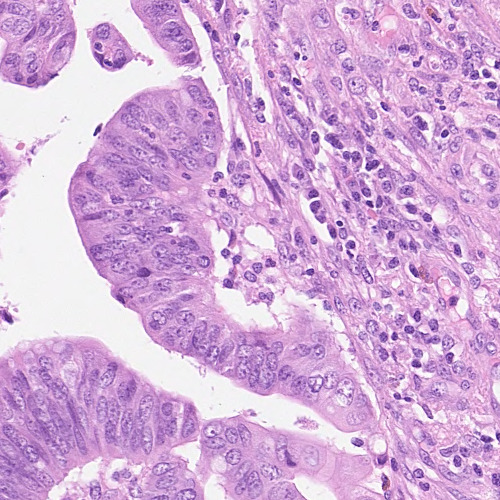
\includegraphics[width=0.9\linewidth]{region1.jpg}
	\end{subfigure}
	\begin{subfigure}{0.3\textwidth}
		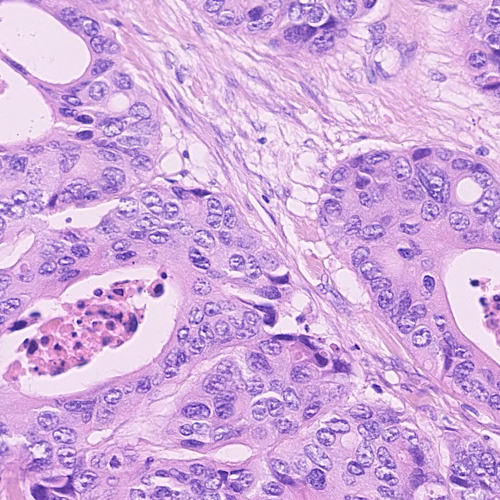
\includegraphics[width=0.9\linewidth]{region2.jpg}
	\end{subfigure}
	\begin{subfigure}{0.3\textwidth}
		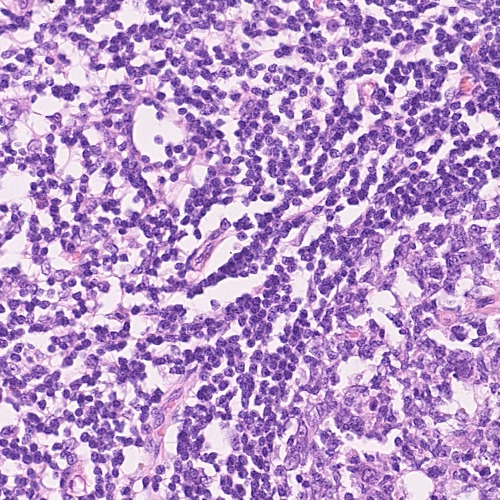
\includegraphics[width=0.9\linewidth]{region3.jpg}
	\end{subfigure}
	\caption{Three example regions from the CRCHistoPhenotypes dataset~\cite{sirinukunwattana2016locality} with multiple nuclei that will be extracted into patches and augmented.}
	\label{fig:region_example}
\end{figure}

\subsection{Training Parameters}
This experiment used a simple CNN inspired by the architecture used in the nuclei classification benchmark for the CRCHistoPhenotypes dataset~\cite{sirinukunwattana2016locality}. It consisted of two convolutional layers, one with 36 filters with a size of 4x4 and the other with 48 filters with a size of 3x3, both of which were followed by max pooling layers with a filter size of 2x2. These layers were followed by two fully connected layers with 1200 neurons and 512 neurons respectively. This architecture is summarised in Table~\ref{tab:cnn}. Each hidden layer used ReLU activation functions and the two fully connected layers used dropout for regularisation~\cite{srivastava2014dropout}. Dropout was also used to adapt the CNN into a Bayesian CNN.

\begin{table}[b!]
	\centering
	\begin{tabular}{|c|c|c}
		\hline
		\multicolumn{3}{|c|}{\begin{tabular}[c]{@{}c@{}}Convolutional Neural Network Architecture \\ for Nuclei Classification\end{tabular}} \\ \hline
		Type & \begin{tabular}[c]{@{}c@{}}Filter\\ Dimensions\end{tabular} & \multicolumn{1}{c|}{\begin{tabular}[c]{@{}c@{}}Input/Output\\ Dimensions\end{tabular}} \\ \hline
		I &  & \multicolumn{1}{c|}{30 x 30 x 3} \\ \hline
		C & 4 x 4 x 1 x 36 & \multicolumn{1}{c|}{26 x 26 x 36} \\ \hline
		M & 2 x 2 & \multicolumn{1}{c|}{12 x 12 x 36} \\ \hline
		C & 3 x 3 x 36 x 48 & \multicolumn{1}{c|}{10 x 10 x 48} \\ \hline
		M & 2 x 2 & \multicolumn{1}{c|}{5 x 5 x 48} \\ \hline
		F & 5 x 5 x 48 x 1200 & \multicolumn{1}{c|}{1 x 1200} \\ \hline
		F & 1 x 1 x 512 x 512 & \multicolumn{1}{c|}{1 x 512} \\ \hline
		F & 1 x 1 x 512 x 4 & \multicolumn{1}{c|}{1 x 4} \\ \hline
	\end{tabular}
	\caption{The Convolutional Neural Network architecture for nuclei classification used in the region-based active learning experiments.}
	\label{tab:cnn}
\end{table}

The training environment is constantly changing between iterations as the  dataset expands. The Adadelta training algorithm for gradient decent was chosen as the CNN’s training optimiser~\cite{zeiler2012adadelta}. Adadelta requires no manual tuning of learning rate as it adapts based on the training gradients, making it ideal for active learning tasks. To ensure that the model has been trained after each active iteration and that overfitting have been avoided, an early stopping method was used. The early stopping method chosen compares the generalisation loss (Equation \ref{eq:generalization_loss}) and training progression (Equation \ref{eq:training_progression}) and will stop training before overfitting~\cite{prechelt1998early}. Generalisation loss is calculated by comparing the validation loss for each epoch \(L_{val}(t)\) against the minimum validation loss across all epochs. The training progression value is calculated by analysing the training losses \(L_{tr}(t)\) over a batch of recent epochs of size \(k\).

\begin{equation}
	GL(t) = 100 \cdot \left ( \frac{L_{va}(t)}{\underset{t'\leq t}{min}L_{va}(t')} - 1 \right )
	\label{eq:generalization_loss}
\end{equation}
\begin{equation}
	P_k(t) = 1000 \cdot \left ( \frac{\sum_{t'=t-k+1}^{t}L_{tr}(t')}{k \cdot min^{t}_{t'=t-k+1}L_{tr}(t')} - 1\right )
	\label{eq:training_progression}
\end{equation}

\subsection{Experiment Setup}
Experiments tested the region-based modification combined with a range of query strategies. These query strategies included several more basic methods which will be used specifically to act as baselines for the other query strategies, built specifically for deep learning algorithms. These basic query strategies are random, least confident uncertainty, margin uncertainty and entropy uncertainty sampling. The other query strategies tried were K-Centre sampling (solved using a greedy approximation), Core-Set sampling~\cite{sener2018active} and Bayesian active learning by disagreement (BALD) sampling using Bayesian neural networks~\cite{gal2017deep}. 

In each experiment, all available data were initially treated as unannotated; two randomly selected regions were then used to form the initial annotated training set. After each active iteration, two regions were selected from the unannotated regions to be added to the training set. This was continued for 50 iterations meaning that 102 regions out of 2,500 formed the final training set in each experiment. Each experimental setting was run five times with different random seeds (different weight initialisation and initial annotated patches). 

\subsection{Results}
Table~\ref{tab:query_results} gives the test accuracy and loss (averaged over the five runs) after 50 iterations for each of the query strategies. These results were obtained on a single, unchanging test set. Notably, only K-Centre sampling achieved a higher average accuracy than a random sampling strategy. Core-set sampling accuracy was very similar to that of random sampling. The other query strategies were all worse than simply adopting random sampling. Figs.~\ref{fig:accuracy} and~\ref{fig:loss} show the test accuracy and loss for each strategy after each iteration. 

For comparison, a fully supervised CNN trained on a much larger training set of 2,500 annotated regions achieved an accuracy of 68.53\% and a loss of 1.111. Training using the K-Centre query strategy achieved an accuracy of 61.41\% and a loss of 1.137 using 4\% of the annotations. 


\begin{table}[ht!]
	\centering
	\begin{tabular}{l|lllllll}
		\begin{tabular}[c]{@{}l@{}}Query \\ Strategy\end{tabular} & Random & \begin{tabular}[c]{@{}l@{}}Least\\ Confident\end{tabular} & Margin & Entropy & K-Centre & Core-Set & BALD \\ \hline
		\multicolumn{1}{l|}{Accuracy} & 58.25\% & 48.92\% & 45.84\% & 32.37\% & 61.41\% & 57.33\% & 48.23\% \\
		\multicolumn{1}{l|}{Loss} & 1.154 & 1.243 & 1.268 & 1.39 & 1.123 & 1.157 & 1.247
	\end{tabular}
	\caption{The accuracy and loss for each model trained with different query strategies over 50 iterations resulting in a total of 102 annotated regions.}
	\label{tab:query_results}
\end{table}



\section{Conclusion}
This paper proposed a mechanism for applying deep active learning to patch-based systems with a specific focus on its application to nuclei classification. The results clearly showed that the traditional active learning query strategies performed poorly. Active learning methods tailored to deep CNNs are needed. Reducing annotation overheads and thus the cost of developing deep learning systems for digital pathology and medical image analysis can allow those with less access to resources to work on a range of problems. Methods such as active learning have great potential but further work is needed in order to achieve significant gains on tasks such as that investigated here. 
